%\documentstyle[epsf,twocolumn]{jarticle}       %LaTeX2e仕様
\documentclass[twocolumn]{jarticle}     %pLaTeX2e仕様(platex.exeの場合)
% \documentclass[onecolumn]{ujarticle}   %pLaTeX2e仕様(uplatex.exeの場合)
%%%%%%%%%%%%%%%%%%%%%%%%%%%%%%%%%%%%%%%%%%%%%%%%%%%%%%%%%%%%%%
%%
%%  基本バージョン
%%
%%%%%%%%%%%%%%%%%%%%%%%%%%%%%%%%%%%%%%%%%%%%%%%%%%%%%%%%%%%%%%%%
\setlength{\topmargin}{-45pt}
%\setlength{\oddsidemargin}{0cm}
\setlength{\oddsidemargin}{-7.5mm}
%\setlength{\evensidemargin}{0cm}
\setlength{\textheight}{24.1cm}
%setlength{\textheight}{25cm}
\setlength{\textwidth}{17.4cm}
%\setlength{\textwidth}{172mm}
\setlength{\columnsep}{11mm}

%\kanjiskip=.07zw plus.5pt minus.5pt


% 【節が変わるごとに (1.1)(1.2) … (2.1)(2.2) と数式番号をつけるとき】
%\makeatletter
%\renewcommand{\theequation}{%
%\thesection.\arabic{equation}} %\@addtoreset{equation}{section}
%\makeatother

%\renewcommand{\arraystretch}{0.95} 行間の設定
%%%%%%%%%%%%%%%%%%%%%%%%%%%%%%%%%%%%%%%%%%%%%%%%%%%%%%%%
%\usepackage{graphicx}   %pLaTeX2e仕様(\documentstyle ->\documentclass)
\usepackage[dvipdfmx]{graphicx}
\usepackage{subcaption}
\usepackage{multirow}
\usepackage{amsmath}
\usepackage{url}
\usepackage{ulem}
\usepackage{algorithm}
\usepackage{algorithmic}
\usepackage{listings} %,jlisting} %日本語のコメントアウトをする場合jlistingが必要
%ここからソースコードの表示に関する設定
\lstset{
  basicstyle={\ttfamily},
  identifierstyle={\small},
  commentstyle={\smallitshape},
  keywordstyle={\small\bfseries},
  ndkeywordstyle={\small},
  stringstyle={\small\ttfamily},
  frame={tb},
  breaklines=true,
  columns=[l]{fullflexible},
  numbers=left,
  xrightmargin=0zw,
  xleftmargin=3zw,
  numberstyle={\scriptsize},
  stepnumber=1,
  numbersep=1zw,
  lineskip=-0.5ex
}
%%%%%%%%%%%%%%%%%%%%%%%%%%%%%%%%%%%%%%%%%%%%%%%%%%%%%%%%
\begin{document}

	%bibtex用の設定
	%\bibliographystyle{ujarticle}

	\twocolumn[
		\noindent
		\hspace{1em}
		2020 年 7 月 31 日
		ゼミ資料
		\hfill
		B4 杉山 竜弥
		\vspace{2mm}

		\hrule
		\begin{center}
			{\Large \bf 進捗報告}
		\end{center}
		\hrule
		\vspace{9mm}
	]

	% ‚ここから 文章 Start!
\section{今週やったこと}
\begin{itemize}
	\item {NASの実装}
\end{itemize}

\section{NAS}
\subsection{設定}
表\ref{tab:setting}には実験設定を示した.
入力・出力ノードの数は, ともに1に設定した.
また出力ノードへの接続はチャンネルのconcatであり, 今回は2つのノードを使ってチャンネル数を2倍にした.
ノードは7にしたため, 探索する辺は15となった.
表\ref{tab:ops}のように, 畳み込み層, プーリング層, 恒等写像, 零写像の6つの演算子を用意した.
またセルの入力は, チャンネル数の前処理としてPointwise Convolutionを用いた.

このセルを4つ重ねたものを用いて, Cifar10の10クラス分類器を構築した.
モデルのOptimizerはSGDで, アーキテクチャを表す\thetaはAdamとした.

\begin{table}[tb]
  \begin{center}
    \caption{実験の設定}
    \begin{tabular}{|c|c|} \hline
      Cell & 5 \\ \hline
      Node & 7(input=1, output=1) \\ \hline
      Optim(model) & SGD(lr=1e-2, momentum=0.9) \\ \hline
      Optim($\theta$) & Adam(lr=2e-4, $\beta$=(0.5, 0.999)) \\ \hline
      Loss & Cross Entropy Loss \\ \hline
      batch size & 64 \\ \hline
      train data & 20000 \\ \hline
      epoch & 10+80+90 \\ \hline
    \end{tabular}
    \label{tab:setting}
  \end{center}
\end{table}

\begin{table}[tb]
  \begin{center}
    \caption{演算子候補}
    \begin{tabular}{|c|} \hline
      \verb|conv_3x3| \\ \hline
      \verb|conv_5x5| \\ \hline
      \verb|avg_pool_3x3| \\ \hline
      \verb|max_pool_3x3| \\ \hline
      \verb|skip_connect| \\ \hline
      \verb|none| \\ \hline
    \end{tabular}
    \label{tab:ops}
  \end{center}
\end{table}

\subsection{変更点}
今回は各ノードが最大2つの親を持つように設定し, モデルの複雑化をした.
Reduction Cellを実装し, 画像サイズを半分にするセルを2番目, 4番目のセルとして追加した.

\subsection{実験}
実験ではまず\thetaを固定して演算子ごとの重みだけを(a)10 epoch学習し,
その後\thetaも加えて(b)60 epoch訓練した.
得られた\thetaからセルの構造を決定し, 重みを(c)90 epochで再学習した.
図\ref{fig:acc}に精度を示した.
訓練時間は全体でおよそ2時間程度であった.

\begin{figure}[tb]
	\begin{center}
		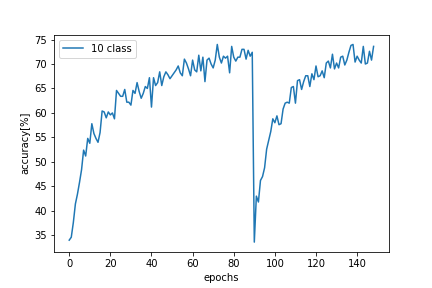
\includegraphics[clip,width=7.5cm]{accuracy.png}
		\caption{テスト精度}
		\label{fig:acc}
	\end{center}
\end{figure}

図\ref{fig:cell}, \ref{fig:cell2}に得られたセルを示した.

\begin{figure*}[t]
	\begin{center}
		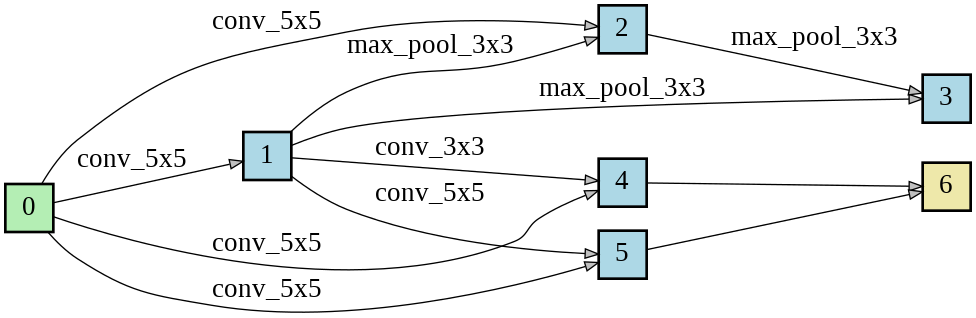
\includegraphics[clip,width=12.5cm]{completenormal.png}
		\caption{Normal Cell}
		\label{fig:cell}
	\end{center}
\end{figure*}

\begin{figure*}[t]
	\begin{center}
		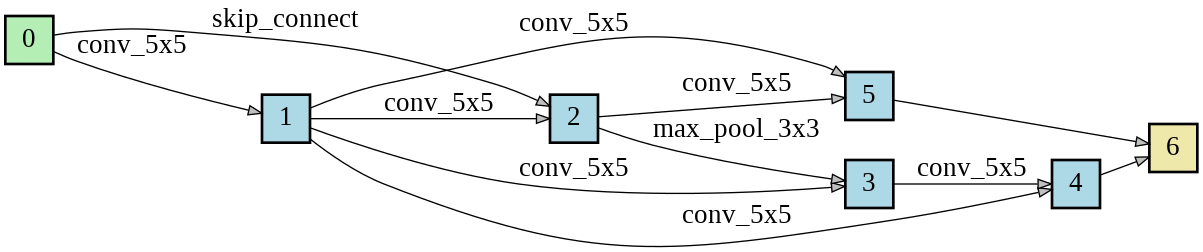
\includegraphics[clip,width=14.5cm]{completereduce.png}
		\caption{Reduction Cell}
		\label{fig:cell2}
	\end{center}
\end{figure*}

\section{考察}
Cellの構造をある程度複雑にできるようになった.
対して精度は手作業で設計したほうがいい精度である.

暫定的に設定していた表\ref{tab:ops}の演算子には非線形性がないため, どれだけ重ねても精度が上がらないと考えられる.
活性化関数の扱いを調査して, 新たな演算子の追加をしたい.

\section{今後の予定}
% なんとなくなんかの勉強をするとかではなく具体的に
\begin{itemize}
  \item 演算子を増やす
  \item セルの多入力の対応
\end{itemize}

\section{ソースコード}
% 埋め込みでもGitでもいいので参照できるように
Githubの同階層の\url{NAS_test.ipynb}を参照してください.

% 参考文献リスト
\bibliographystyle{unsrt}
\bibliography{ref}
\end{document}
